\documentclass[12pt]{article}
\setlength{\oddsidemargin}{0in}
\setlength{\evensidemargin}{0in}
\setlength{\textwidth}{6.5in}
\setlength{\parindent}{0in}
\setlength{\parskip}{\baselineskip}

\usepackage[letterpaper, portrait, margin=1in]{geometry}
\usepackage[usenames, dvipsnames, rgb]{xcolor}
\usepackage{amsmath,amsfonts,amssymb,circuitikz,pdfpages,tikz,fancyvrb}
\usepackage{tikz-timing}

\usetikzlibrary{matrix,calc,shapes.geometric,circuits.logic.US,positioning}
\tikzstyle{mux} = [ trapezium,   draw,
                    shape border rotate = 270, trapezium angle = 60,
                    inner ysep=0pt, outer sep=1pt, inner xsep=1pt,
                    text width = 1.5em, align = center,
                    node distance=3cm]
\tikzstyle{branch}=[fill, shape=circle, minimum size=3pt, inner sep=0pt]

%isolated term
%#1 - Optional. Space between node and grouping line. Default=0
%#2 - node
%#3 - filling color
\newcommand{\implicantsol}[3][0]{
    \draw[rounded corners=3pt, fill=#3, opacity=0.3] ($(#2.north west)+(135:#1)$) rectangle ($(#2.south east)+(-45:#1)$);
    }


%internal group
%#1 - Optional. Space between node and grouping line. Default=0
%#2 - top left node
%#3 - bottom right node
%#4 - filling color
\newcommand{\implicant}[4][0]{
    \draw[rounded corners=3pt, fill=#4, opacity=0.3] ($(#2.north west)+(135:#1)$) rectangle ($(#3.south east)+(-45:#1)$);
    }

%group lateral borders
%#1 - Optional. Space between node and grouping line. Default=0
%#2 - top left node
%#3 - bottom right node
%#4 - filling color
\newcommand{\implicantcostats}[4][0]{
    \draw[rounded corners=3pt, fill=#4, opacity=0.3] ($(rf.east |- #2.north)+(90:#1)$)-| ($(#2.east)+(0:#1)$) |- ($(rf.east |- #3.south)+(-90:#1)$);
    \draw[rounded corners=3pt, fill=#4, opacity=0.3] ($(cf.west |- #2.north)+(90:#1)$) -| ($(#3.west)+(180:#1)$) |- ($(cf.west |- #3.south)+(-90:#1)$);
}

%group top-bottom borders
%#1 - Optional. Space between node and grouping line. Default=0
%#2 - top left node
%#3 - bottom right node
%#4 - filling color
\newcommand{\implicantdaltbaix}[4][0]{
    \draw[rounded corners=3pt, fill=#4, opacity=0.3] ($(cf.south -| #2.west)+(180:#1)$) |- ($(#2.south)+(-90:#1)$) -| ($(cf.south -| #3.east)+(0:#1)$);
    \draw[rounded corners=3pt, fill=#4, opacity=0.3] ($(rf.north -| #2.west)+(180:#1)$) |- ($(#3.north)+(90:#1)$) -| ($(rf.north -| #3.east)+(0:#1)$);
}

%group corners
%#1 - Optional. Space between node and grouping line. Default=0
%#2 - filling color
\newcommand{\implicantcantons}[2][0]{
    \draw[rounded corners=3pt, opacity=.3] ($(rf.east |- 0.south)+(-90:#1)$) -| ($(0.east |- cf.south)+(0:#1)$);
    \draw[rounded corners=3pt, opacity=.3] ($(rf.east |- 8.north)+(90:#1)$) -| ($(8.east |- rf.north)+(0:#1)$);
    \draw[rounded corners=3pt, opacity=.3] ($(cf.west |- 2.south)+(-90:#1)$) -| ($(2.west |- cf.south)+(180:#1)$);
    \draw[rounded corners=3pt, opacity=.3] ($(cf.west |- 10.north)+(90:#1)$) -| ($(10.west |- rf.north)+(180:#1)$);
    \fill[rounded corners=3pt, fill=#2, opacity=.3] ($(rf.east |- 0.south)+(-90:#1)$) -|  ($(0.east |- cf.south)+(0:#1)$) [sharp corners] ($(rf.east |- 0.south)+(-90:#1)$) |-  ($(0.east |- cf.south)+(0:#1)$) ;
    \fill[rounded corners=3pt, fill=#2, opacity=.3] ($(rf.east |- 8.north)+(90:#1)$) -| ($(8.east |- rf.north)+(0:#1)$) [sharp corners] ($(rf.east |- 8.north)+(90:#1)$) |- ($(8.east |- rf.north)+(0:#1)$) ;
    \fill[rounded corners=3pt, fill=#2, opacity=.3] ($(cf.west |- 2.south)+(-90:#1)$) -| ($(2.west |- cf.south)+(180:#1)$) [sharp corners]($(cf.west |- 2.south)+(-90:#1)$) |- ($(2.west |- cf.south)+(180:#1)$) ;
    \fill[rounded corners=3pt, fill=#2, opacity=.3] ($(cf.west |- 10.north)+(90:#1)$) -| ($(10.west |- rf.north)+(180:#1)$) [sharp corners] ($(cf.west |- 10.north)+(90:#1)$) |- ($(10.west |- rf.north)+(180:#1)$) ;
}

%Empty Karnaugh map 4x4
\newenvironment{Karnaugh}%
{
\begin{tikzpicture}[baseline=(current bounding box.north),scale=0.8]
\draw (0,0) grid (4,4);
\draw (0,4) -- node [pos=1,above right,anchor=south west] {$x_2 x_3$} node [pos=0.7,below left,anchor=north east] {$x_0 x_1$} ++(135:1);
%
\matrix (mapa) [matrix of nodes,
        column sep={0.8cm,between origins},
        row sep={0.8cm,between origins},
        every node/.style={minimum size=0.3mm},
        anchor=8.center,
        ampersand replacement=\&] at (0.5,0.5)
{
                       \& |(c00)| 00         \& |(c01)| 01         \& |(c11)| 11         \& |(c10)| 10         \& |(cf)| \phantom{00} \\
|(r00)| 00             \& |(0)|  \phantom{0} \& |(1)|  \phantom{0} \& |(3)|  \phantom{0} \& |(2)|  \phantom{0} \&                     \\
|(r01)| 01             \& |(4)|  \phantom{0} \& |(5)|  \phantom{0} \& |(7)|  \phantom{0} \& |(6)|  \phantom{0} \&                     \\
|(r11)| 11             \& |(12)| \phantom{0} \& |(13)| \phantom{0} \& |(15)| \phantom{0} \& |(14)| \phantom{0} \&                     \\
|(r10)| 10             \& |(8)|  \phantom{0} \& |(9)|  \phantom{0} \& |(11)| \phantom{0} \& |(10)| \phantom{0} \&                     \\
|(rf) | \phantom{00}   \&                    \&                    \&                    \&                    \&                     \\
};
}%
{
\end{tikzpicture}
}

%Empty Karnaugh map 4x4
\newenvironment{Karnaugh5}%
{
\begin{tikzpicture}[baseline=(current bounding box.north),scale=0.8]
\draw (0,0) grid (4,4);
\draw (0,4) -- node [pos=1,above right,anchor=south west] {$x_4x_5$} node [pos=0.7,below left,anchor=north east] {$x_2x_3$} ++(135:1);
%
\matrix (mapa) [matrix of nodes,
        column sep={0.8cm,between origins},
        row sep={0.8cm,between origins},
        every node/.style={minimum size=0.3mm},
        anchor=8.center,
        ampersand replacement=\&] at (0.5,0.5)
{
                       \& |(c00)| 00         \& |(c01)| 01         \& |(c11)| 11         \& |(c10)| 10         \& |(cf)| \phantom{00} \\
|(r00)| 00             \& |(0)|  \phantom{0} \& |(1)|  \phantom{0} \& |(3)|  \phantom{0} \& |(2)|  \phantom{0} \&                     \\
|(r01)| 01             \& |(4)|  \phantom{0} \& |(5)|  \phantom{0} \& |(7)|  \phantom{0} \& |(6)|  \phantom{0} \&                     \\
|(r11)| 11             \& |(12)| \phantom{0} \& |(13)| \phantom{0} \& |(15)| \phantom{0} \& |(14)| \phantom{0} \&                     \\
|(r10)| 10             \& |(8)|  \phantom{0} \& |(9)|  \phantom{0} \& |(11)| \phantom{0} \& |(10)| \phantom{0} \&                     \\
|(rf) | \phantom{00}   \&                    \&                    \&                    \&                    \&                     \\
};
}%
{
\end{tikzpicture}
}

%Empty Karnaugh map 2x4
\newenvironment{Karnaughvuit}%
{
\begin{tikzpicture}[baseline=(current bounding box.north),scale=0.8]
\draw (0,0) grid (4,2);
\draw (0,2) -- node [pos=1,above right,anchor=south west] {$x_2x_3$} node [pos=0.7,below left,anchor=north east] {$x_1$} ++(135:1);
%
\matrix (mapa) [matrix of nodes,
        column sep={0.8cm,between origins},
        row sep={0.8cm,between origins},
        every node/.style={minimum size=0.3mm},
        anchor=4.center,
        ampersand replacement=\&] at (0.5,0.5)
{
                      \& |(c00)| 00         \& |(c01)| 01         \& |(c11)| 11         \& |(c10)| 10         \& |(cf)| \phantom{00} \\
|(r00)| 0             \& |(0)|  \phantom{0} \& |(1)|  \phantom{0} \& |(3)|  \phantom{0} \& |(2)|  \phantom{0} \&                     \\
|(r01)| 1             \& |(4)|  \phantom{0} \& |(5)|  \phantom{0} \& |(7)|  \phantom{0} \& |(6)|  \phantom{0} \&                     \\
|(rf) | \phantom{00}  \&                    \&                    \&                    \&                    \&                     \\
};
}%
{
\end{tikzpicture}
}

%Empty Karnaugh map 2x2
\newenvironment{Karnaughquatre}%
{
\begin{tikzpicture}[baseline=(current bounding box.north),scale=0.8]
\draw (0,0) grid (2,2);
\draw (0,2) -- node [pos=0.7,above right,anchor=south west] {b} node [pos=0.7,below left,anchor=north east] {a} ++(135:1);
%
\matrix (mapa) [matrix of nodes,
        column sep={0.8cm,between origins},
        row sep={0.8cm,between origins},
        every node/.style={minimum size=0.3mm},
        anchor=2.center,
        ampersand replacement=\&] at (0.5,0.5)
{
          \& |(c00)| 0          \& |(c01)| 1  \\
|(r00)| 0 \& |(0)|  \phantom{0} \& |(1)|  \phantom{0} \\
|(r01)| 1 \& |(2)|  \phantom{0} \& |(3)|  \phantom{0} \\
};
}%
{
\end{tikzpicture}
}

%Defines 8 or 16 values (0,1,X)
\newcommand{\contingut}[1]{%
\foreach \x [count=\xi from 0]  in {#1}
     \path (\xi) node {\x};
}

%Places 1 in listed positions
\newcommand{\minterms}[1]{%
    \foreach \x in {#1}
        \path (\x) node {1};
}

%Places 0 in listed positions
\newcommand{\maxterms}[1]{%
    \foreach \x in {#1}
        \path (\x) node {0};
}


\newcommand{\overbar}[1]
    {\mkern1.5mu\overline{\mkern-1.5mu#1\mkern-1.5mu}\mkern1.5mu}

\begin{document}

\renewcommand{\arraystretch}{1}

\makeatletter
    \pgfdeclareshape{JK}{
      \savedanchor\northeast{%
        \pgfmathsetlength\pgf@x{\pgfshapeminwidth}%
        \pgfmathsetlength\pgf@y{\pgfshapeminheight}%
        \pgf@x=0.5\pgf@x
        \pgf@y=0.5\pgf@y
      }
      % This is redundant, but makes some things easier:
      \savedanchor\southwest{%
        \pgfmathsetlength\pgf@x{\pgfshapeminwidth}%
        \pgfmathsetlength\pgf@y{\pgfshapeminheight}%
        \pgf@x=-0.5\pgf@x
        \pgf@y=-0.5\pgf@y
      }
      \inheritsavedanchors[from=rectangle]
      \inheritanchorborder[from=rectangle]
      \anchor{center}{\pgfpointorigin}
      \anchor{north}{\northeast \pgf@x=0pt}
      \anchor{east}{\northeast \pgf@y=0pt}
      \anchor{south}{\southwest \pgf@x=0pt}
      \anchor{west}{\southwest \pgf@y=0pt}
      \anchor{north east}{\northeast}
      \anchor{north west}{\northeast \pgf@x=-\pgf@x}
      \anchor{south west}{\southwest}
      \anchor{south east}{\southwest \pgf@x=-\pgf@x}
      \anchor{J}{
        \pgf@process{\northeast}%
        \pgf@x=-1\pgf@x%
        \pgf@y=.5\pgf@y%
      }
      \anchor{CLK}{
        \pgf@process{\northeast}%
        \pgf@x=-1\pgf@x%
        \pgf@y=0\pgf@y%
      }
      \anchor{K}{
        \pgf@process{\northeast}%
        \pgf@x=-1\pgf@x%
        \pgf@y=-0.5\pgf@y%
      }
      \anchor{Q}{
        \pgf@process{\northeast}%
        \pgf@y=.5\pgf@y%
      }
      \anchor{Qn}{
        \pgf@process{\northeast}%
        \pgf@y=-.5\pgf@y%
      }

      \backgroundpath{
        % Rectangle box
        \pgfpathrectanglecorners{\southwest}{\northeast}
        % Angle (>) for clock input
        \pgf@anchor@JK@CLK
        \pgf@xa=\pgf@x \pgf@ya=\pgf@y
        \pgf@xb=\pgf@x \pgf@yb=\pgf@y
        \pgf@xc=\pgf@x \pgf@yc=\pgf@y
        \pgfmathsetlength\pgf@x{1.6ex} % size depends on font size
        \advance\pgf@ya by \pgf@x
        \advance\pgf@xb by \pgf@x
        \advance\pgf@yc by -\pgf@x
        \pgfpathmoveto{\pgfpoint{\pgf@xa}{\pgf@ya}}
        \pgfpathlineto{\pgfpoint{\pgf@xb}{\pgf@yb}}
        \pgfpathlineto{\pgfpoint{\pgf@xc}{\pgf@yc}}
        \pgfclosepath

        \begingroup

        \pgf@anchor@JK@K
        \pgftext[left,base,at={\pgfpoint{\pgf@x}{\pgf@y}},
          x=\pgfshapeinnerxsep]{\raisebox{-0.75ex}{K}}


        \pgf@anchor@JK@J
        \pgftext[left,base,at={\pgfpoint{\pgf@x}{\pgf@y}},
          x=\pgfshapeinnerxsep]{\raisebox{-0.75ex}{J}}

        \pgf@anchor@JK@Q
        \pgftext[right,base,at={\pgfpoint{\pgf@x}{\pgf@y}},
          x=-\pgfshapeinnerxsep]{\raisebox{-.75ex}{Q}}

        \pgf@anchor@JK@Qn
        \pgftext[right,base,at={\pgfpoint{\pgf@x}{\pgf@y}},
          x=-\pgfshapeinnerxsep]{\raisebox{-.75ex}{$\overline{\mbox{Q}}$}}

        \endgroup
      }
    }
    % Key to add font macros to the current font
    \tikzset{add font/.code={\expandafter\def\expandafter\tikz@textfont
            \expandafter{\tikz@textfont#1}}}

    % Define default style for this node
    \tikzset{flip flop/port labels/.style={font=\sffamily\scriptsize}}
    \tikzset{every JK node/.style={draw,minimum width=1.5cm,
            minimum height=2.25cm,inner sep=1mm,outer sep=0pt,
            cap=round,add font=\sffamily}}
\makeatother

\makeatletter
    \pgfdeclareshape{tff}{
      \savedanchor\northeast{%
        \pgfmathsetlength\pgf@x{\pgfshapeminwidth}%
        \pgfmathsetlength\pgf@y{\pgfshapeminheight}%
        \pgf@x=0.5\pgf@x
        \pgf@y=0.5\pgf@y
      }
      % This is redundant, but makes some things easier:
      \savedanchor\southwest{%
        \pgfmathsetlength\pgf@x{\pgfshapeminwidth}%
        \pgfmathsetlength\pgf@y{\pgfshapeminheight}%
        \pgf@x=-0.5\pgf@x
        \pgf@y=-0.5\pgf@y
      }
      \inheritsavedanchors[from=rectangle]
      \inheritanchorborder[from=rectangle]
      \anchor{center}{\pgfpointorigin}
      \anchor{north}{\northeast \pgf@x=0pt}
      \anchor{east}{\northeast \pgf@y=0pt}
      \anchor{south}{\southwest \pgf@x=0pt}
      \anchor{west}{\southwest \pgf@y=0pt}
      \anchor{north east}{\northeast}
      \anchor{north west}{\northeast \pgf@x=-\pgf@x}
      \anchor{south west}{\southwest}
      \anchor{south east}{\southwest \pgf@x=-\pgf@x}
      \anchor{T}{
        \pgf@process{\northeast}%
        \pgf@x=-1\pgf@x%
        \pgf@y=.5\pgf@y%
      }
      \anchor{CLK}{
        \pgf@process{\northeast}%
        \pgf@x=-1\pgf@x%
        \pgf@y=-.5\pgf@y%
      }
      \anchor{Q}{
        \pgf@process{\northeast}%
        \pgf@y=.5\pgf@y%
      }
      \anchor{Qn}{
        \pgf@process{\northeast}%
        \pgf@y=-.5\pgf@y%
      }

      \backgroundpath{
        % Rectangle box
        \pgfpathrectanglecorners{\southwest}{\northeast}
        % Angle (>) for clock input
        \pgf@anchor@tff@CLK
        \pgf@xa=\pgf@x \pgf@ya=\pgf@y
        \pgf@xb=\pgf@x \pgf@yb=\pgf@y
        \pgf@xc=\pgf@x \pgf@yc=\pgf@y
        \pgfmathsetlength\pgf@x{1.6ex} % size depends on font size
        \advance\pgf@ya by \pgf@x
        \advance\pgf@xb by \pgf@x
        \advance\pgf@yc by -\pgf@x
        \pgfpathmoveto{\pgfpoint{\pgf@xa}{\pgf@ya}}
        \pgfpathlineto{\pgfpoint{\pgf@xb}{\pgf@yb}}
        \pgfpathlineto{\pgfpoint{\pgf@xc}{\pgf@yc}}
        \pgfclosepath

        \begingroup

        \pgf@anchor@tff@T
        \pgftext[left,base,at={\pgfpoint{\pgf@x}{\pgf@y}},
          x=\pgfshapeinnerxsep]{\raisebox{-0.75ex}{T}}

        \pgf@anchor@tff@Q
        \pgftext[right,base,at={\pgfpoint{\pgf@x}{\pgf@y}},
          x=-\pgfshapeinnerxsep]{\raisebox{-.75ex}{Q}}

        \pgf@anchor@tff@Qn
        \pgftext[right,base,at={\pgfpoint{\pgf@x}{\pgf@y}},
          x=-\pgfshapeinnerxsep]{\raisebox{-.75ex}{$\overline{\mbox{Q}}$}}

        \endgroup
      }
    }
    % Key to add font macros to the current font
    \tikzset{add font/.code={\expandafter\def\expandafter\tikz@textfont
            \expandafter{\tikz@textfont#1}}}

    % Define default style for this node
    \tikzset{flip flop/port labels/.style={font=\sffamily\scriptsize}}
    \tikzset{every tff node/.style={draw,minimum width=1.5cm,
            minimum height=2.25cm,inner sep=1mm,outer sep=0pt,
            cap=round,add font=\sffamily}}
\makeatother

\makeatletter
    \pgfdeclareshape{dff}{
      \savedanchor\northeast{%
        \pgfmathsetlength\pgf@x{\pgfshapeminwidth}%
        \pgfmathsetlength\pgf@y{\pgfshapeminheight}%
        \pgf@x=0.5\pgf@x
        \pgf@y=0.5\pgf@y
      }
      % This is redundant, but makes some things easier:
      \savedanchor\southwest{%
        \pgfmathsetlength\pgf@x{\pgfshapeminwidth}%
        \pgfmathsetlength\pgf@y{\pgfshapeminheight}%
        \pgf@x=-0.5\pgf@x
        \pgf@y=-0.5\pgf@y
      }
      \inheritsavedanchors[from=rectangle]
      \inheritanchorborder[from=rectangle]
      \anchor{center}{\pgfpointorigin}
      \anchor{north}{\northeast \pgf@x=0pt}
      \anchor{east}{\northeast \pgf@y=0pt}
      \anchor{south}{\southwest \pgf@x=0pt}
      \anchor{west}{\southwest \pgf@y=0pt}
      \anchor{north east}{\northeast}
      \anchor{north west}{\northeast \pgf@x=-\pgf@x}
      \anchor{south west}{\southwest}
      \anchor{south east}{\southwest \pgf@x=-\pgf@x}
      \anchor{D}{
        \pgf@process{\northeast}%
        \pgf@x=-1\pgf@x%
        \pgf@y=.5\pgf@y%
      }
      \anchor{CLK}{
        \pgf@process{\northeast}%
        \pgf@x=-1\pgf@x%
        \pgf@y=-.5\pgf@y%
      }
      \anchor{Q}{
        \pgf@process{\northeast}%
        \pgf@y=.5\pgf@y%
      }
      \anchor{Qn}{
        \pgf@process{\northeast}%
        \pgf@y=-.5\pgf@y%
      }

      \backgroundpath{
        % Rectangle box
        \pgfpathrectanglecorners{\southwest}{\northeast}
        % Angle (>) for clock input
        \pgf@anchor@dff@CLK
        \pgf@xa=\pgf@x \pgf@ya=\pgf@y
        \pgf@xb=\pgf@x \pgf@yb=\pgf@y
        \pgf@xc=\pgf@x \pgf@yc=\pgf@y
        \pgfmathsetlength\pgf@x{1.6ex} % size depends on font size
        \advance\pgf@ya by \pgf@x
        \advance\pgf@xb by \pgf@x
        \advance\pgf@yc by -\pgf@x
        \pgfpathmoveto{\pgfpoint{\pgf@xa}{\pgf@ya}}
        \pgfpathlineto{\pgfpoint{\pgf@xb}{\pgf@yb}}
        \pgfpathlineto{\pgfpoint{\pgf@xc}{\pgf@yc}}
        \pgfclosepath

        \begingroup

        \pgf@anchor@dff@D
        \pgftext[left,base,at={\pgfpoint{\pgf@x}{\pgf@y}},
          x=\pgfshapeinnerxsep]{\raisebox{-0.75ex}{D}}

        \pgf@anchor@dff@Q
        \pgftext[right,base,at={\pgfpoint{\pgf@x}{\pgf@y}},
          x=-\pgfshapeinnerxsep]{\raisebox{-.75ex}{Q}}

        \pgf@anchor@dff@Qn
        \pgftext[right,base,at={\pgfpoint{\pgf@x}{\pgf@y}},
          x=-\pgfshapeinnerxsep]{\raisebox{-.75ex}{$\overline{\mbox{Q}}$}}

        \endgroup
      }
    }
    % Key to add font macros to the current font
    \tikzset{add font/.code={\expandafter\def\expandafter\tikz@textfont
            \expandafter{\tikz@textfont#1}}}

    % Define default style for this node
    \tikzset{flip flop/port labels/.style={font=\sffamily\scriptsize}}
    \tikzset{every dff node/.style={draw,minimum width=1.5cm,
            minimum height=2.25cm,inner sep=1mm,outer sep=0pt,
            cap=round,add font=\sffamily}}
\makeatother

\title{Digital Logic Homework 8}

ECEN 2350 Spring 2017 \hfill Homework 8\\
Samuel Cuthbertson

\hrulefill{}
\begin{enumerate}
  \item \textit{Book Problems: 6.9, 6.11}
  \begin{enumerate}
    \item[6.9:] \textit{A sequential circuit has two inputs, $w_1$ and $w_2$, and an output $z$. Its function is to compare the input sequences on the two inputs. If $w_1 = w_2$ during any four consecutive clock cycles, the circuit produces $z=1$; otherwise, $z=0$. Derive a suitable circuit.}

    As we are looking to detect \textit{any} four consecutive clock cycles, we will only need five states, as shown below in the graph and state diagram. Encoding states as $A=00001$, $B=00010$, $C=00100$, $D=01000$, and $E=10000$, as well as using $w_1 \oplus w_2$ will simplify the below table.

    \begin{center}
      \begin{minipage}{0.4\textwidth}
        \begin{center}
          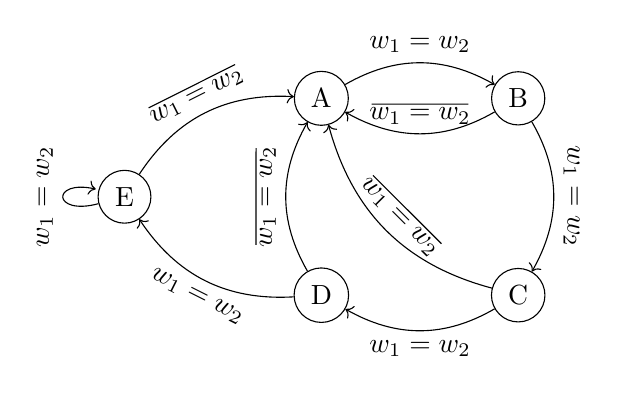
\begin{tikzpicture}[scale=1.25]
            \node[circle, draw] (A) at (0,2) {A};
            \node[circle, draw] (B) at (2,2) {B};
            \node[circle, draw] (C) at (2,0) {C};
            \node[circle, draw] (D) at (0,0) {D};
            \node[circle, draw] (E) at (-2,1) {E};

            \draw[->] (A) edge[bend left] node[above]{$w_1= w_2$} (B);
            \draw[->] (B) edge[bend left] node[above, sloped]{$w_1 = w_2$} (C);
            \draw[->] (C) edge[bend left] node[below]{$w_1 = w_2$} (D);
            \draw[->] (D) edge[bend left] node[below, sloped]{$w_1 = w_2$} (E);

            \draw[->] (E) edge[loop left] node[above, sloped] {$w_1 = w_2$}(E);

            \draw[->] (E) edge[bend left] node[above, sloped]{$\overbar{w_1 = w_2}$} (A);
            \draw[->] (D) edge[bend left] node[above, sloped]{$\overbar{w_1 = w_2}$} (A);
            \draw[->] (C) edge[bend left] node[above, sloped]{$\overbar{w_1 = w_2}$} (A);
            \draw[->] (B) edge[bend left] node[above, sloped]{$\overbar{w_1 = w_2}$} (A);

          \end{tikzpicture}
        \end{center}
      \end{minipage}
      \hfill
      \begin{minipage}{0.4\textwidth}
        \begin{center}
          \begin{tabular}{c|c||c|c}
            S & $w_1 \oplus w_2$ & N & $z$ \\
            \hline
            \hline
            00001 & 0 & 00010 & 0 \\
            00010 & 0 & 00100 & 0 \\
            00100 & 0 & 01000 & 0 \\
            01000 & 0 & 10000 & 1 \\
            10000 & 0 & 10000 & 1 \\
            x & 1 & 00001 & 0 \\
          \end{tabular}
        \end{center}
      \end{minipage}
    \end{center}

    Using the above state table, we can see that each digit $i$ of $N$ is equal to $1$ if and only if $S_{i-1} = 1$ and $w_0 \oplus w_1 = 0$. The exceptions here would be $N_0$, which equals $w_0 \oplus w_1$ and $N_4$ which would equal $S_3\overbar{(w_0 \oplus w_1)} + S_4\overbar{(w_0 \oplus w_1)}$. All other digits would follow the form $N_i = S_{i-1}\overbar{(w_0 \oplus w_1)}$.


    Finally, it's fairly obvious in the above scheme that $z=N_4$, as $N_4 = 1$ only when the next state is E, exactly the same as z. The circuit derived from the above is as follows:

    \begin{center}
      \begin{tikzpicture}[scale=0.75, every node/.style={transform shape}]
        \node[shape=dff](S0) at (0,0) {};
        \node[shape=dff](S1) at (4,0) {};
        \node[shape=dff](S2) at (8,0) {};
        \node[shape=dff](S3) at (12,0) {};
        \node[shape=dff](S4) at (16,0) {};

        \node (clk) at (-1.15,-3) {Clock};
        \draw (clk) |- (S0.CLK);
        \draw (clk) -- ++(4,0) node[branch](clk1){} |- (S1.CLK);
        \draw (clk1) -- ++(4,0) node[branch](clk2){} |- (S2.CLK);
        \draw (clk2) -- ++(4,0) node[branch](clk3){} |- (S3.CLK);
        \draw (clk3) -- ++(4,0) |- (S4.CLK);

        \node[xnor gate US, draw, logic gate inputs = nn] (x) at (0,3) {};
        \node (W0) at (-1.2,3.25) {$w_0$};
        \node (W1) at (-1.2,2.75) {$w_1$};
        \draw (W0) -- ++(0.5,0) |- (x.input 1);
        \draw (W1) -- ++(0.5,0) |- (x.input 2);
        \draw (x.output) -- ++(1,0) -- ++(0,-1.5) node[branch](x1){};
        \node[not gate US, draw, logic gate inputs = n, left = 1.75 of x1, rotate=180](n0){};
        \draw (x1) -- (n0.input);
        \draw (n0.output) -- ++(-0.75,0) |- (S0.D);

        \draw (x1) -- ++(4,0) node[branch](x2){};
        \draw (x2) -- ++(4,0) node[branch](x3){};
        \draw (x3) -- ++(3.6,0) node[branch](x4){};

        \node[and gate US, draw, logic gate inputs = nn, left = 0.5 of S1.D] (N1) {};
        \draw (S0.Q) -- ++(.5,0) |- (N1.input 2);
        \draw (x1) |- (N1.input 1);
        \draw (N1.output) -- (S1.D);

        \node[and gate US, draw, logic gate inputs = nn, left = 0.5 of S2.D] (N2) {};
        \draw (S1.Q) -- ++(.5,0) |- (N2.input 2);
        \draw (x2) |- (N2.input 1);
        \draw (N2.output) -- (S2.D);

        \node[and gate US, draw, logic gate inputs = nn, left = 0.5 of S3.D] (N3) {};
        \draw (S2.Q) -- ++(.5,0) |- (N3.input 2);
        \draw (x3) |- (N3.input 1);
        \draw (N3.output) -- (S3.D);

        \node[and gate US, draw, logic gate inputs = nn, below left = 0.01 and 1.25 of S4.D] (N4) {};
        \draw (S3.Q) -- ++(.25,0) |- (N4.input 2);
        \draw (x4) |- (N4.input 1);
        \node[or gate US, draw, logic gate inputs = nn, left = 0.25 of S4.D] (O4) {};
        \draw (O4.output) -- (S4.D);
        \draw (N4) -- ++(.45,0) |- (O4.input 2);
        \node[and gate US, draw, logic gate inputs = nn, above left = 0.25 and 1.25 of S4.D] (N4a) {};
        \draw (N4a.input 2) -- ++(-.27,0) node[branch]{};
        \draw (S4.Q) -- ++(.25,0) -- ++(0,1.25) -- ++(-3.7,0) |- (N4a.input 1);

      \end{tikzpicture}
    \end{center}

    \newpage
    \item[6.11:] \textit{A given FSM has an input, $w$, and an output, $z$. During four consecutive clock pulses, a sequence of four values of the $w$ signal is applied. Derive a state table for the FSM that produces $z=1$ when it detects that either the sequence $w:0010$ or $w:1110$ has been applied; otherwise, $z=0$. After the fourth clock pulse, the machince has to be again in the reset state, ready for the next sequence. Minimize the number of states needed.}

    Using a very similar approach to above, we can use the state table shown below.

        \begin{center}
          \begin{tabular}{c||c|c|c}
            State & \multicolumn{2}{|c|}{Next State} & z \\
            & $w=0$ & $w=1$ &&
            \hline
            A & B & E & 0 \\
            B & C & A & 0 \\
            C & A & D & 0 \\
            D & H & A & 0 \\
            E & A & F & 0 \\
            F & A & G & 0 \\
            G & H & A & 0 \\
            H & B & E & 1 \\
          \end{tabular}

    \end{center}

    We can then use partitioning as follows:
    \begin{align*}
      P_1 &= (ABCDEFGH)\\
      P_2 &= (ABCDEFG)(H)\\
      P_3 &= (A)(B)(C)(D)(E)(F)(G)(H)
    \end{align*}
    And thus our minimum number of states is eight.
  \end{enumerate}

  \newpage
  \item \textit{Book Problem: B.2}
  \begin{enumerate}
    \item[a:] \textit{Show that the circuit in Figure PB.2 is fuctionally equivalent to the circuit in Figure PB.1.}

    Figure PB.1 is simple to examine, as it is just a cannonical sum-of-products implmenetation. It's formula is $f = \overbar{x_1}\overbar{x_2}x_3 + \overbar{x_1}x_2\overbar{x_3} + x_1\overbar{x_2}\overbar{x_3} + x_1x_2x_3$. Figure PB.2 is best to examine as a look up table, where $x_2$ is the selector in the first layer and $x_1$ is the selector in the second layer. Looking at it as such, we can say that when $x_1x_2$ is true, our circuit will return $x_3$, and when $x_1\overbar{x_2}$ is true our circuit will return $\overbar{x_3}$, etc. This all comes out to $f = \overbar{x_1}\overbar{x_2}x_3 + \overbar{x_1}x_2\overbar{x_3} + x_1\overbar{x_2}\overbar{x_3} + x_1x_2x_3$, which is the exact same as our other circuit.

    \item[b:] \textit{How many transistors are needed to build the CMOS circuit in PB.2? Draw the CMOS circuit.}

    Using the transmission gates desribed on page 787 of the textbook, we can implement the multiplexer circuit as shown:

  \end{enumerate}

  \newpage
  \item \textit{Book Problem: B.7}
  \begin{enumerate}
    \item[a:] \textit{Give the truth table for the CMOS circuit in the Figure PB.5.}
    \begin{center}
      \begin{tabular}{cccc|c}
        $x_0$ & $x_1$ & $x_2$ & $x_3$ & f \\
        \hline
        0 & 0 & 0 & 0 & 1 \\
        0 & 0 & 0 & 1 & 0 \\
        0 & 0 & 1 & 0 & 0 \\
        0 & 0 & 1 & 1 & 0 \\
        0 & 1 & 0 & 0 & 1 \\
        0 & 1 & 0 & 1 & 0 \\
        0 & 1 & 1 & 0 & 0 \\
        0 & 1 & 1 & 1 & 0 \\
        1 & 0 & 0 & 0 & 1 \\
        1 & 0 & 0 & 1 & 0 \\
        1 & 0 & 1 & 0 & 0 \\
        1 & 0 & 1 & 1 & 0 \\
        1 & 1 & 0 & 0 & 0 \\
        1 & 1 & 0 & 1 & 0 \\
        1 & 1 & 1 & 0 & 0 \\
        1 & 1 & 1 & 1 & 0 \\

      \end{tabular}
    \end{center}

    \item[b:] \textit{Derive the simplest sum-of-products expression for the truth table in (a). How many transistors are needed to build the sum-of-products circuit using the CMOS AND, OR and NOT gates?}
    \begin{Karnaugh}
      \contingut{1,0,0,0,1,0,0,0,1,0,0,0,0,0,0,0}
      \implicant{0}{4}{red};
      \implicantsol{8}{orange};
    \end{Karnaugh}\\
    And therefor the simplest SOP expression is $f = \overbar{x_0}\overbar{x_2}\overbar{x_3} + x_0\overbar{x_1}\overbar{x_2}\overbar{x_3}$. As one NOT gate takes 2 transitors, a two input OR gate takes 6 transistors, a four input AND gate takes 10 transistors, and a 3 input AND gate takes 8 transistors, we can sum up the above into:
    \[
    f = 2*4 + 6 + 10 + 8 = \boxed{32}
    \]

  \end{enumerate}

  \newpage
  \item \textit{Given the following schematic from the Texas Instruments CMOS BCD to 7-segment decoder CD4511B, estimate the number of transistors this circuit needs. You cannot ignore the FlipFlops at the inputs to the circuit (the box that is labeled as a PTGN). These are toggle flip flops with preset/clear. Model these like the example from class.}\\
  Assuming the following:
  \begin{itemize}
    \item{Each NAND or NOR gate uses 2n transistors, where n is the number of inputs.}
    \item{A NOT gate is 2 transistors.}
    \item{Each flip flop is composed of an NOT, two ANDs, and an OR gate around a D-Flip Flop with Preset/Clear. Cost of $2+(4+2)+(4+2)+(4+2)+DFF$}
    \item{The cost of a D-Flip-Flop with Preset/Clear is six NAND gates with three inputs, or 36.}
  \end{itemize}

  With all of the the above assumptions, we can see that the circuit contains:

  \begin{itemize}
    \item{22 NOT gates}
    \item{8 T-Flip-Flops}
    \item{6 4-Input NORs}
    \item{8 3-Input NORs}
    \item{12 2-Input NORs and NANDs}
    \item{4 Transitors in the ``Driver Logic''}
  \end{itemize}

  All this sums to:
  \[
    22*2 + 8*56 + 6*4 + 8*3 + 12*2 + 4 = \boxed{568}
  \]

  But this could all vary drastically depending on many factors, such as which implementation one choses for D-Flip-Flops. I picked the one on Page 262 of the textbook.



\end{enumerate}
\end{document}
